\begin{figure*}[!ht]
    \centering
    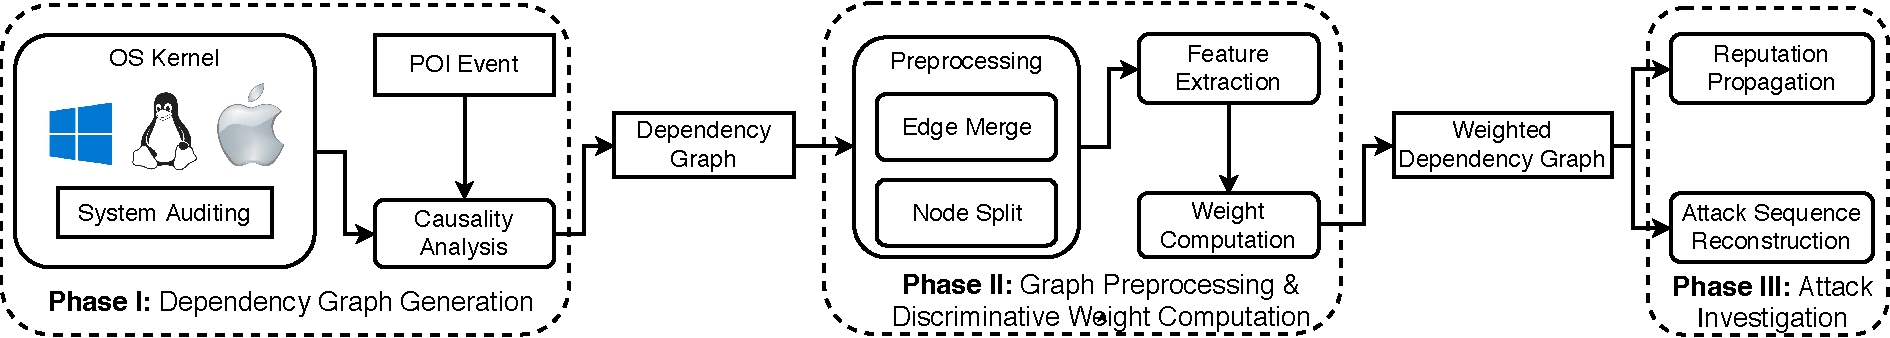
\includegraphics[width=0.98\textwidth,clip]{figs/architecture.pdf}
  %  \vspace{3mm}
    \caption{The architecture of \tool}
  %  \vspace{2mm}
    \label{fig:overview}
%    \vspace*{-1ex}
\end{figure*}


\section{Overview and Threat Model}
\label{sec:overview}

% https://drive.google.com/file/d/1HKHxWAoQWrw-ZGfvF3AJuEUhGcIF-BCy/view?usp=sharing
\cref{fig:overview} illustrates the architecture of \tool. 
\tool consists of three phases: (1) dependency graph generation, (2) graph preprocessing \& discriminative weight computation, and (3) attack investigation.
In Phase I, 
\tool leverages mature system auditing tools (\eg auditd~\cite{auditd}, ETW~\cite{etw}, DTrace~\cite{dtrace}, and Sysdig~\cite{sysdig}) to collect system-level audit logs about system calls.
Given a POI event, \tool parses the collected logs and performs causality analysis~\cite{backtracking,backtracking2} to generate the dependency graph for the event (\cref{subsec:graph-generation}).
%
In Phase II, \tool preprocesses the graph by merging the same type of edges between two nodes that occur within a time window threshold to reduce the graph size and splitting the nodes to remove parallel edges. 
This process transforms the large dependency graph into a simple directed graph (\cref{subsec:graph-preprocessing}), which is easier for weight computation and reputation propagation.
To produce a weighted dependency graph such that critical edges
%(\ie edges that reveal the attack provenance) 
are easily distinguishable from non-critical edges by their weights, for each edge, \tool extracts three novel features that model the importance of the event edge w.r.t. the POI event from three dimensions: time dimension, data amount dimension, and structure dimension (\cref{subsec:feature-extraction}). 
\tool then employs a novel \emph{local feature projection mechanism} to project the three features to a combined, discriminative weight (\cref{subsec:weight-computation}).
%
In Phase III, \tool enables automatic attack investigation by (1) propagating reputation from seeds sources on the weighted dependency graph to automatically determine the suspiciousness/trustworthiness of POI entities (\cref{subsec:attack-investigation})
and (2) providing a suggested range of threshold values based on the discriminative edge weights to automatically reconstruct attack sequence by distinguishing critical edges from other edges.


\eat{
The main steps of the proposed framework can be summarized as follows: (i) System auditing tools are deployed on the host. (ii) System call activities are collected by the auditing tools and stored. (iii) A dependency graph is built out of the monitoring data and causality analysis is applied to reconstruct the time line of a given vertex of security significance. (iv) The graph is trimmed by merging redundant edges. (v) Vertices are split if there exists parallel edges. (vi) After these prepossessing steps, the weight of each edge in the graph is computed. (vii) Based on the weights, the reputation score of the system entity of interest in the graph is inferred by reputation propagation. (viii) Non-critical edges can be further pruned to achieve better human readability of the graph. Figure~\ref{fig:after} shows a sample dependency graph after the whole process of \tool. }



\myparatight{Threat Model}
Our threat model follows the threat model of previous work on system monitoring~\cite{backtracking,backtracking2,loggc,trustkernel,gao2018aiql,gao2018saql,liu2018priotracker,hassan2019nodoze}. 
We assume that the system monitoring data collected from kernel space~\cite{auditd,etw,dtrace,sysdig} is not tampered, and that the kernel is trusted.
Any kernel-level attack that deliberately compromises security auditing systems is beyond the scope of this work.

\eat{
The attacker executes APT attacks involving multiple steps such as target discovery and data exfiltration. We assume an outside attacker that attacks the system remotely (from outside of the system). Thus, the attacker either utilizes the vulnerabilities in the system or convinces the user to download a file. The main goal of the attacker is to inject her malicious files into the victim’s system without being detected. In this work, we assume the attacker does not know how the proposed reputation system operates, and hence we do not consider the potential attacks against the reputation system. 
}


% We do consider that insiders or external attackers have full knowledge of the deployed \tool queries and the anomaly models. 